% !TEX TS-program = pdflatex
% !TEX encoding = UTF-8 Unicode

% This is a simple template for a LaTeX document using the "article" class.
% See "book", "report", "letter" for other types of document.

\documentclass[11pt]{article} % use larger type; default would be 10pt

\usepackage[utf8]{inputenc} % set input encoding (not needed with XeLaTeX)

%%% PAGE DIMENSIONS
\usepackage{geometry} % to change the page dimensions
\geometry{a4paper} % or letterpaper (US) or a5paper or....

\usepackage{graphicx} % support the \includegraphics command and options

\usepackage{amssymb}
\usepackage{amsmath}
%%% PACKAGES
\usepackage{booktabs} % for much better looking tables
\usepackage{array} % for better arrays (eg matrices) in maths
\usepackage{paralist} % very flexible & customisable lists (eg. enumerate/itemize, etc.)
\usepackage{verbatim} % adds environment for commenting out blocks of text & for better verbatim
\usepackage{subfig} % make it possible to include more than one captioned figure/table in a single float
% These packages are all incorporated in the memoir class to one degree or another...

%%% HEADERS & FOOTERS
\usepackage{fancyhdr} % This should be set AFTER setting up the page geometry
\pagestyle{fancy} % options: empty , plain , fancy
\renewcommand{\headrulewidth}{0pt} % customise the layout...
\lhead{}\chead{}\rhead{}
\lfoot{}\cfoot{\thepage}\rfoot{}

%%% SECTION TITLE APPEARANCE
\usepackage{sectsty}
\allsectionsfont{\sffamily\mdseries\upshape} % (See the fntguide.pdf for font help)
% (This matches ConTeXt defaults)

%%% ToC (table of contents) APPEARANCE
\usepackage[nottoc,notlof,notlot]{tocbibind} % Put the bibliography in the ToC
\usepackage[titles,subfigure]{tocloft} % Alter the style of the Table of Contents
\renewcommand{\cftsecfont}{\rmfamily\mdseries\upshape}
\renewcommand{\cftsecpagefont}{\rmfamily\mdseries\upshape} % No bold!
\usepackage{graphicx}
\graphicspath{ {./pings/} }

\usepackage{amsmath}
\DeclareMathOperator*{\argmax}{arg\,max}
\DeclareMathOperator*{\argmin}{arg\,min}

\newcount\colveccount
\newcommand*\colvec[1]{
        \global\colveccount#1
        \begin{pmatrix}
        \colvecnext
}
\def\colvecnext#1{
        #1
        \global\advance\colveccount-1
        \ifnum\colveccount>0
                \\
                \expandafter\colvecnext
        \else
                \end{pmatrix}
        \fi
}

%%% END Article customizations

%%% The "real" document content comes below...

\title{Macro PS3}
\author{Michael B. Nattinger\footnote{I worked on this assignment with my study group: Alex von Hafften, Andrew Smith, and Ryan Mather. I have also discussed problem(s) with Emily Case, Sarah Bass, and Danny Edgel.}}

%\date{} % Activate to display a given date or no date (if empty),
         % otherwise the current date is printed 

\begin{document}
\maketitle

\section{Question 1}
We study a similar environment to the OG model we studied in class. We now assume no commitment technology and we assume allocations $w_1,w_2$ in each generation's second period. 
\subsection{State and solve the planner's problem.}
The planner maximizes utility subject to the resource constraints:
\begin{align}
\begin{split}
&\max_{c_{t}^{t-1},c_{t}^{t}} \text{ln } c_{t}^{t-1} + \text{ln } c_{t}^{t}\\  \label{eqn:planner}
&\text{s.t. } c_{t}^{t-1} + c_{t}^{t} \leq w_1 + w_2.
\end{split}
\end{align}

Since utility is strictly increasing in consumption, the resource constraint will hold with equality so we can solve for $c_t^t$ in terms of $c_t^{t+1}:$ $c_t^t = w_1 + w_2 - c_t^{t+1}.$ Then we can rewrite the maximization problem as the following:

\begin{align*}
&\max_{c_{t}^{t-1}} \text{ln } c_{t}^{t-1} + \text{ln } (w_1 + w_2 - c_t^{t-1})\\
&\Rightarrow \frac{1}{c_{*,t}^{t-1}} - \frac{1}{w_1 + w_2 - c_t^{*,t-1}} = 0\\
&\Rightarrow c_t^{*,t-1} = \frac{w_1 + w_2}{2} \\
&\Rightarrow c_t^{*,t} = \frac{w_1 + w_2}{2}.
\end{align*}

Thus, the social planner will set $c_t^{*,t-1} = c_t^{*,t} = \frac{w_1 + w_2}{2}$.

\subsection{State the representative household's problem in period $t \geq 0$.}
The households maximize utility subject to their budget constraints:
\begin{align*}
\begin{split}
&\max_{c_{t}^{t},c_{t+1}^{t},M_{t+1}^t} \text{ln } c_{t}^{t} + \text{ln } c_{t+1}^{t}\\ 
&\text{s.t. } p_t c_{t}^{t} + M_{t+1}^{t} \leq p_t w_1 \\
&\text{and } p_{t+1} c_{t+1}^{t} \leq p_{t+1} w_2 + M_{t+1}^{t}
\end{split}
\end{align*}
Rewriting the budget constraints,
\begin{align}
\begin{split}
&\max_{c_{t}^{t},c_{t+1}^{t},M_{t+1}^t} \text{ln } c_{t}^{t} + \text{ln } c_{t+1}^{t}\\  \label{eqn:hh}
&\text{s.t. } c_{t}^{t} + \frac{M_{t+1}^{t}}{p_t} \leq w_1 \\
&\text{and }  c_{t+1}^{t} \leq w_2 + \frac{M_{t+1}^{t}}{p_{t+1}}
\end{split}
\end{align}


The initial old generation
 lives only one period and maximizes their utility in that period subject to their budget constraint in that period.
\begin{align*}
\begin{split}
&\max_{c_{1}^{0}} \text{ln } c_{1}^{0}\\ 
&\text{s.t. } p_{1} c_{1}^{0} \leq p_{1} w_2 + M
\end{split}
\end{align*}
Again rewriting the budget constraint,
\begin{align*}
\begin{split}
&\max_{c_{1}^{0}} \text{ln } c_{1}^{0}\\ 
&\text{s.t. } c_{1}^{0} \leq w_2 + \frac{M}{p_1}.
\end{split}
\end{align*}

\subsection{Define and solve for an autarkic equilibrium, assuming it exists.} %Change - money market still has to clear but 1/p_t is 0
In the Autarkic equilibrium, there is no belief that money will have value in the future. Thus, individuals will not trade any of their endowment for money, so  $M$ has no value for the initial old agent. Since utility is strictly increasing in consumption, the budget constraints will hold with equality so we have the following solution: $c_t^{**,t} = w_1, c_{t+1}^{**,t} = w_2$ $\forall i \in \mathbb{N} \cup \{0\}.$ Note that the money market must still clear, so $M_{t+1}^t = M$, but $\frac{M_{t+1}^t}{p_{t}} = \frac{M_{t+1}^t}{p_{t+1}} = 0.$

\subsection{Define and solve for a competitive equilibrium assuming valued money but with $w_2 = 0.$}
Now we will solve for a competitive equilibrium assuming agents will expect money will carry value into the future, and assuming $w_2 = 0.$ Our agents then solve the following:
\begin{align*}
\begin{split}
&\max_{c_{t}^{t},c_{t+1}^{t},M_{t+1}^t} \text{ln } c_{t}^{t} + \text{ln } c_{t+1}^{t}\\  
&\text{s.t. } c_{t}^{t} + \frac{M_{t+1}^{t}}{p_t} \leq w_1 \\
&\text{and }  c_{t+1}^{t} \leq \frac{M_{t+1}^{t}}{p_{t+1}}
\end{split}
\end{align*}
Utility is strictly increasing with consumption so the budget constraints will hold with equality - that is, $c_{t+1}^{t} = \frac{M_{t+1}^{t}}{p_{t+1}}, c_{t}^{t} + \frac{M_{t+1}^{t}}{p_t} = w_1 \Rightarrow c_{t}^{t} = w_1 - \frac{M_{t+1}^{t}}{p_t}  $. We then have:
\begin{align*}
\begin{split}
&\max_{M_{t+1}^t} \text{ln } \left(w_1 - \frac{M_{t+1}^{t}}{p_t}\right) + \text{ln } \frac{M_{t+1}^{t}}{p_{t+1}}
\end{split}
\end{align*}

Taking first order conditions:
\begin{align*}
0 &= -(p_t^{***})^{-1}\frac{1}{w_1 - M_{t+1}^{***,t} / p_t^{***}} + (p_{t+1}^{***})^{-1}\frac{1}{M_{t+1}^{***,t}/p_{t+1}^{***}}\\
\Rightarrow  M_{t+1}^{***,t} &= \frac{p_t^{***} w_1}{2}\\
\Rightarrow c_t^{***,t} &= \frac{w_1}{2}, c_{t+1}^{***,t} = \frac{p_t^{***}}{p_{t+1}^{***}}\frac{w_1}{2}
\end{align*}

In the first period, the initial old solves the following:
\begin{align*}
\begin{split}
&\max_{c_{1}^{0}} \text{ln } c_{1}^{0}\\ 
&\text{s.t. } c_{1}^{0} \leq \frac{M}{p_1}.
\end{split}
\end{align*}
Utility is increasing in consumption so the budget constraint holds with equality: $c_{1}^{***,0} = \frac{M}{p_1^{***}}$.

In the competitive equilibrium, our money market must clear so $M_{t+1}^{***,t} = M \Rightarrow \frac{p_t^{***} w_1}{2} = M \Rightarrow p_t^{***} = \frac{2M}{w_1}$ $\forall t \in \mathbb{N}.$ This value is constant so $p_i^{***} = p_j^{***}$ $\forall i,j \in \mathbb{N}.$ By Walras' law, this also clears the goods market, which we can verify: $c_t^{***,t} + c_t^{***,t-1} = w_1 \Rightarrow \frac{w_1}{2} + \frac{p_{t-1}^{***}}{p_t^{***}}\frac{w_1}{2} = w_1 \Rightarrow w_1 = w_1.$

Therefore, $c_t^{***,t} = c_{t+1}^{***,t} = \frac{w_1}{2}$, $p_t^{***} =  \frac{2M}{w_1}$, $M_{t+1}^{***,t} = M.$

\subsection{Compare the solutions to the planner's problem, the autarky equilibrium, and the stationary monetary competitive equilibrium with valued money, all with $w_2 = 0.$}
The solution to the planner's problem was  $c_t^{*,t-1} = c_t^{*,t} = \frac{w_1 + w_2}{2}$, so for $w_2 = 0$ the solution is $c_t^{*,t-1} = c_t^{*,t} = \frac{w_1}{2} = c_t^{***,t-1} = c_t^{***,t}$ so the solutions for the planner's problem and stationary monetary competitive equilibrium with valued money are equivalent. Note however that, for $w_2 = 0$, $c_t^{**,t} = w_1, c_{t+1}^{**,t} = 0$ which is a strictly worse solution for the agents as this yields $-\infty$ utility in the second period for the agents. Thus, the autarky equilibrium does not yield the same result as the planner's problem.

\subsection{What happens to consumption, money demand, and prices in a competitive equilibrium with valued money if the initial money supply is halved?}
Denote with primes the new values of the variables in the equilibrium with halved money supply.
\begin{equation*}
c_t^{',***,t} = c_{t+1}^{',***,t} = \frac{w_1}{2}, M_{t+1}^{',***,t} = \frac{M}{2}, p_t^{',***,t} =  \frac{M}{w_1}.
\end{equation*}
If the initial money supply is halved, the consumption allocations are unchanged, and the prices and money demand adjust accordingly.

\section{Question 2}
Plot the trade offer curves for the following utility functions where the endowment is $(w_1,w_2)$ for goods 1 and 2, respectively:
\subsection{$U = 10 c_1 - 4 c_{1}^2 + 4c_2 - c_{2}^2, (w_1,w_2) = (0,2)$}
%The agent will trade to (weakly) increase their utility: $U(c_1,c_2)\geq U(w_1,w_2) = 0.$ We will solve for a convenient expression for $c_1,c_2$:
%\begin{align*}
%\Rightarrow& 10 c_1 - 4 c_{1}^2 + 4c_2 - c_{2}^2 \geq 0 \Rightarrow -10 c_1 + 4 c_{1}^2 + (c_2 - 2)^2 \leq 4 \\
%\Rightarrow& 4(c_1 - \frac{5}{4})^2 +  (c_2 - 2)^2 \leq 4 + \frac{25}{4} = \frac{41}{4} \\
%\Rightarrow& \frac{16}{41}(c_1 - \frac{5}{4})^2 +  \frac{4}{41}(c_2 - 2)^2 \leq 1.
%\end{align*}
%It is clear that our expression for $c_1,c_2$ is of the form of a filled ellipse centered at $(\frac{5}{4},2)$ with semi-major axis in the $c_2$ direction with length $\frac{\sqrt{41}}{2}$ and semi-minor axis in the $c_1$ direction with length $\frac{\sqrt{41}}{4}.$ This ellipse is plotted below. Note: $c_1,c_2\geq 0.$
%
%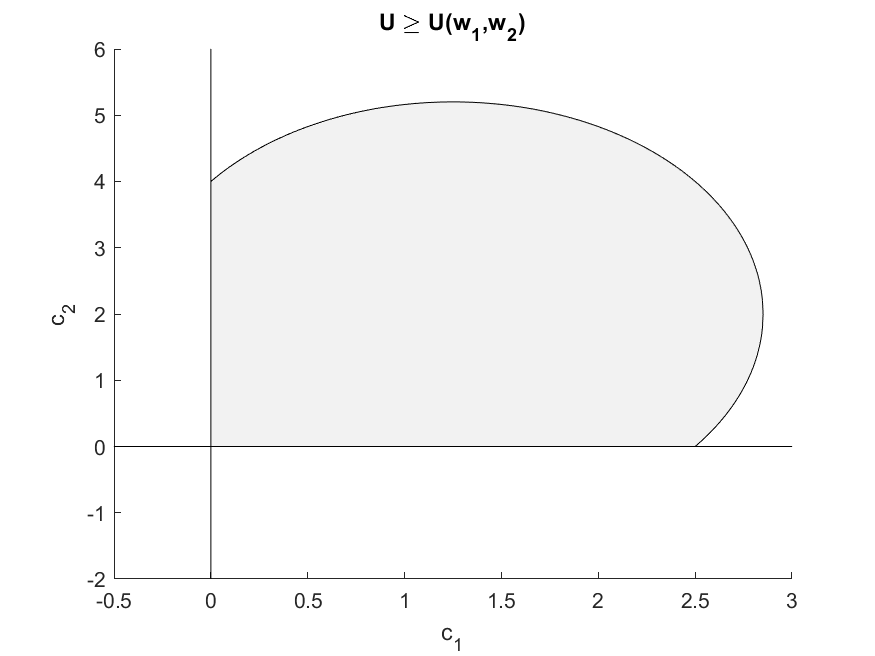
\includegraphics{p1}
Note that our utility curves take the form of ellipses. Fixing U,
\begin{align*}
\Rightarrow& 10 c_1 - 4 c_{1}^2 + 4c_2 - c_{2}^2 = U \Rightarrow -10 c_1 + 4 c_{1}^2 + (c_2 - 2)^2 = 4-U \\
\Rightarrow& 4\left(c_1 - \frac{5}{4}\right)^2 +  (c_2 - 2)^2 = 4 + \frac{25}{4} - U = \frac{41}{4} - U.
\end{align*}
Thus, our utility curves take the form of ellipses centered at (5/4,2), with semi-major and semi-minor axis lengths shrinking to 0 as $U \rightarrow \frac{41}{4}$. Note also that $\frac{\partial U}{\partial c_1} = 0 \Rightarrow c_1^{*} = 5/4, \frac{\partial U}{\partial c_2} = 0 \Rightarrow c_2^{*} = 2$ so not only are our ellipses centered at  (5/4,2), but the global maximum of utility is at that point.

Our initial allocation is $ (w_1,w_2) = (0,2).$ Our budget constraint is the following: $p_1 c_1 + p_2 c_2 = p_1 w_1 + p_2 w_2 = 2p_2 \Rightarrow c_2 = \frac{2p_2 - p_1 c_1}{p_2} = 2 - \frac{p_1}{p_2}c_1.$ We can plug this into our utility and we have the following:
\begin{align*}
U &= 10c_1 - 4c_1^2 + 4\left(2 -  \frac{p_1}{p_2}c_1 \right)- \left(2 -  \frac{p_1}{p_2}c_1 \right)^2 \\
\Rightarrow U &= 10c_1 - 4c_1^2 + 8 - 4\frac{p_1}{p_2}c_1 - 4 + 4\frac{p_1}{p_2}c_1 - \left( \frac{p_1}{p_2}c_1 \right)^2 \\
\Rightarrow U &= 10c_1 - 4c_1^2 + 4 - \left( \frac{p_1}{p_2}c_1 \right)^2
\end{align*}
We can then take a first order condtion with regard to $c_1$: $\frac{\partial U}{\partial c_1} = 0 \Rightarrow \frac{\partial}{\partial c_1} 10c_1 - 4c_1^2 + 4 - \left( \frac{p_1}{p_2}c_1 \right)^2 = 0 \Rightarrow 10 - 8c_1^{**} - 2 \left(\frac{p_1}{p_2}\right)^2c_1^{*} = 0 \Rightarrow c_1^{**} = \frac{10}{8 + 2(p_1/p_2)^2}$
Thus, given a price ratio $p_1/p_2$ we can calculate $c_1^{**} = \frac{10}{8 + 2(p_1/p_2)^2}, c_2^{**} = 2 - \frac{p_1}{p_2}c_1^{**}$.

Below are plots of the budget constraint given different price ratios, and their resulting optimal consumption points and indifference curves at the optimal utility. This traces out the offer curve, with the offer curve being formally drawn with the initial allocation at the origin.

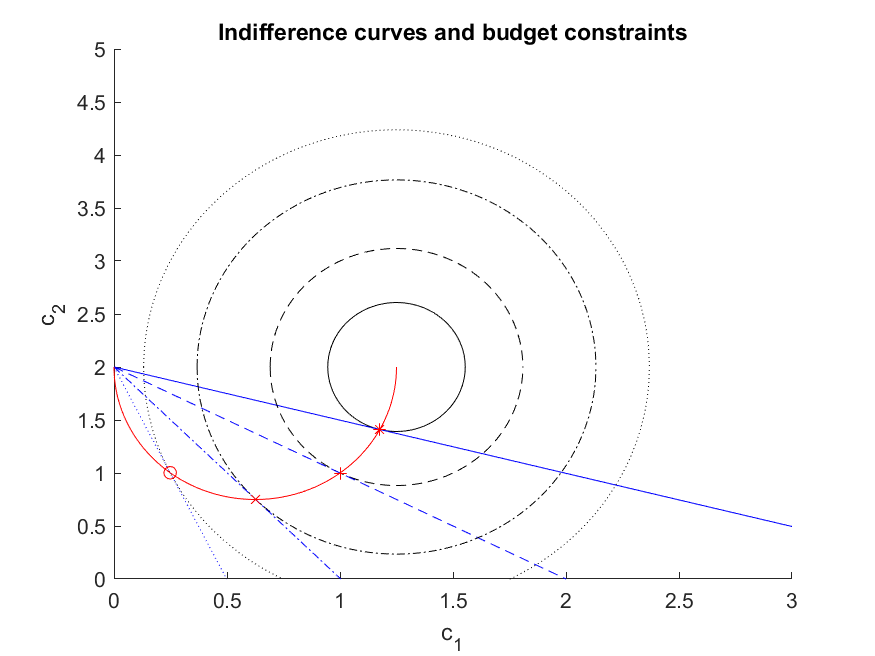
\includegraphics{indiff1}
In the above plot, the black curves indicate indifference curves for the highest possible utility given the price ratio. The blue curves indicate the budget constraints at those ratios, and the red symbols indicate the optimal points on the budget constraints. The red symbols trace out the curve of optimal choices from the agents which, when graphed in deviations from initial allocation, is the offer curve (below).

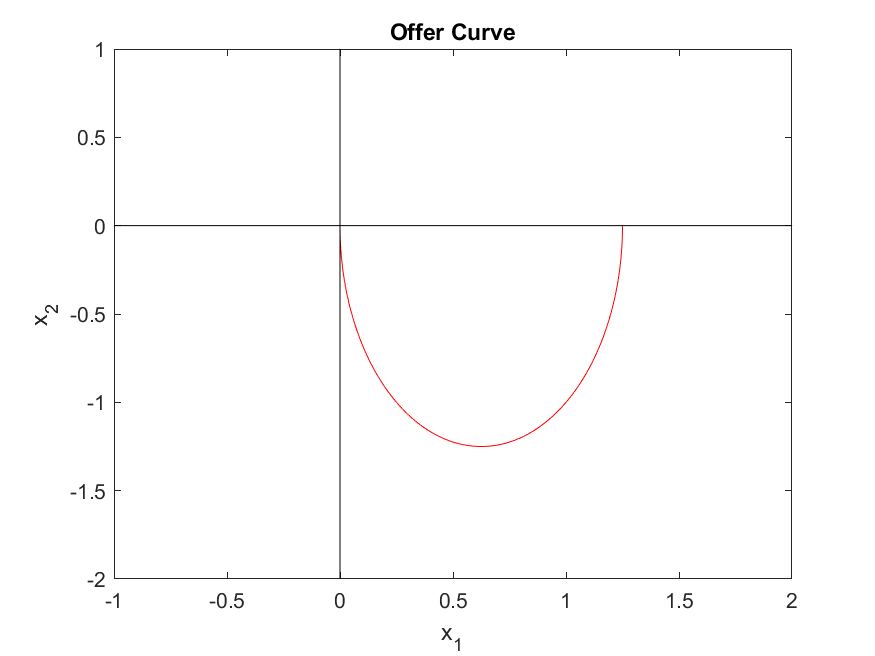
\includegraphics{off1}

\subsection{$U = \min \{ 2c_1 + c_2, c_1 + 2 c_2\}, (w_1,w_2) = (1,0)$}
We begin at our initial allocation, $(w_1,w_2) = (1,0).$ If $p_1 = 0$ then we can increase $c_1$ as much as we would like, so we will consume an infinite amount of it. As $p_1/p_2$ rises, we will stay at our initial allocation until $p_1/p_2$ reaches $1/2$. At this point we will be indifferent between trading for the second consumption good, so we can travel along the curve $c_1 + 2c_2 = w_1 + 2w_2 = 1$ until $c_1 = c_2 = \frac{1}{3}$. As $p_1/p_2$ increases further from there, the optimal choice is to equalize $c_1,c_2$ until $p_1/p_2 = 2$. At this point we will be indifferent between equalizing $c_1,c_2$ (so so $c_1 = c_2 = 2/3$)and traveling to the left along the curve $2c_1 + c_2 = 2w_1 +w_2 = 2$. For $p_1/p_2>2$, we will always trade all of our allocation for $c_2$. This is plotted below.

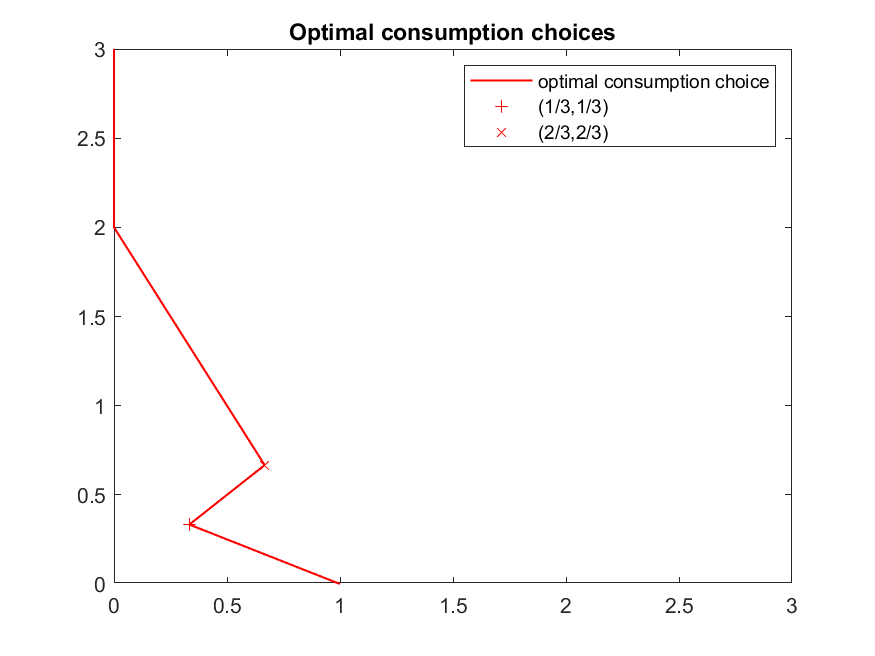
\includegraphics{indiff2}

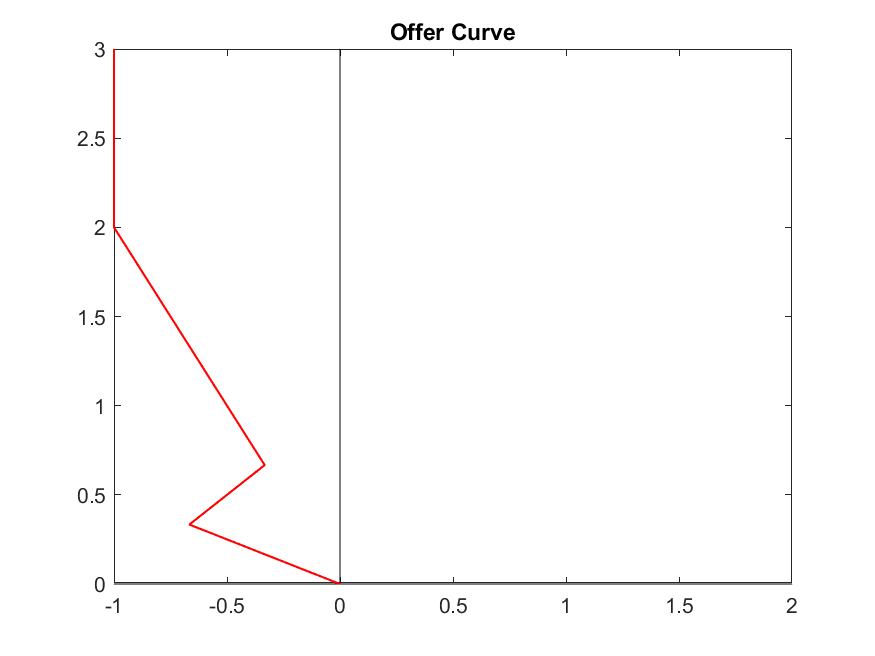
\includegraphics{off2}
%Our agent will trade to (weakly) increase their utility: $U(c_1,c_2)\geq U(w_1,w_2) = 1$. We will solve for a convenient expression for $c_1,c_2$:
%\begin{align*}
%2c_1 + c_2 &\geq 1 \\
%c_1 + 2c_2 &\geq 1 \\
%\Rightarrow  c_2&\geq 1 - 2c_1 \\
%\Rightarrow c_2&\geq \frac{1-c_1}{2}
%\end{align*}
%Thus, our agent will trade to any point which is on or above both curves. This is plotted below. Note: $c_1,c_2\geq 0.$

%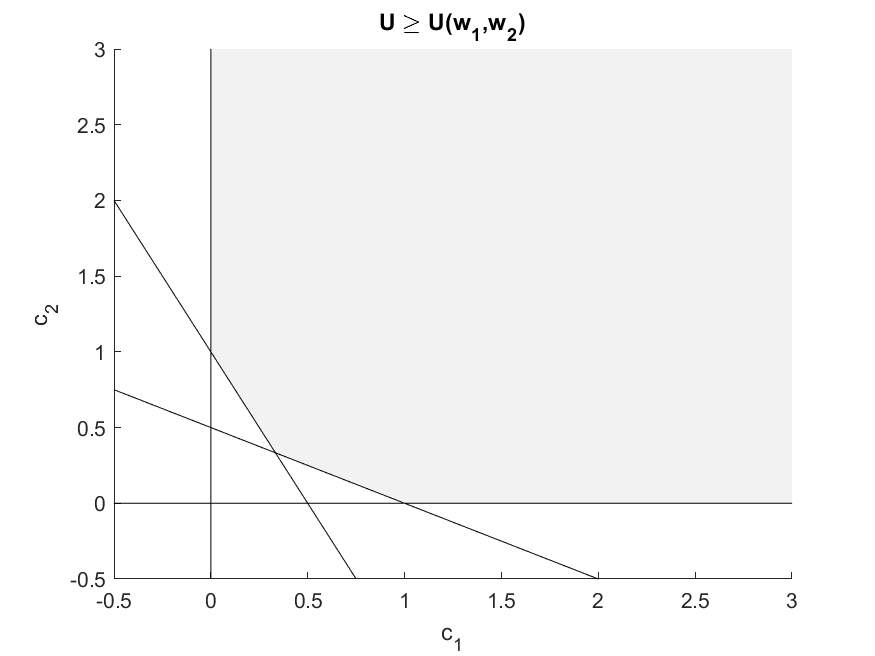
\includegraphics{p2}

\subsection{$U = \min \{ 2c_1 + c_2, c_1 + 2 c_2\}, (w_1,w_2) = (1,10)$}
We begin at our initial allocation, $(w_1,w_2) = (1,10).$ If $p_2 = 0$ then we can increase $c_1$ as much as we would like so we will consume an infinite amount. As $p_2/p_1$ rises, we will consume only good 2 until $p_2/p_1$ reaches $1/2$. At this point we will be indifferent between trading for the first consumption good, so we can travel along the curve $2c_1 + c_2 = 2w_1 + w_2 = 12$ until $c_1 = c_2 = 4$. As $p_2/p_1$ increases further from there, the optimal choice is to equalize $c_1,c_2$ until $p_2/p_1 = 2$. At this point we will be indifferent between equalizing $c_1,c_2$ (so so $c_1 = c_2 = 7$) and traveling to the right along the curve $c_1 +2c_2 = w_1 +2w_2 = 21$. For $p_2/p_1>2$, we will always trade all of our allocation for $c_1$. This is plotted below.

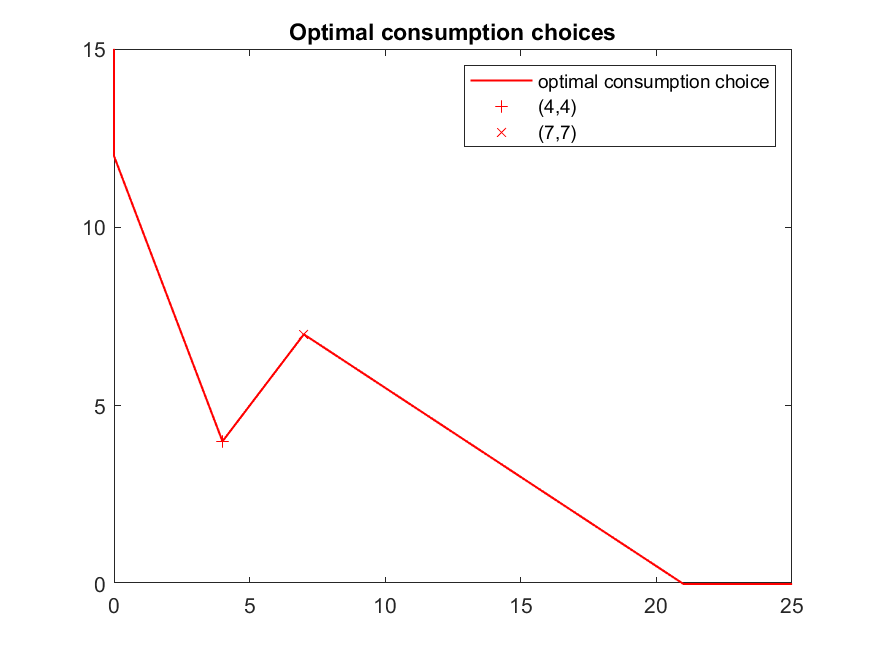
\includegraphics{indiff3}

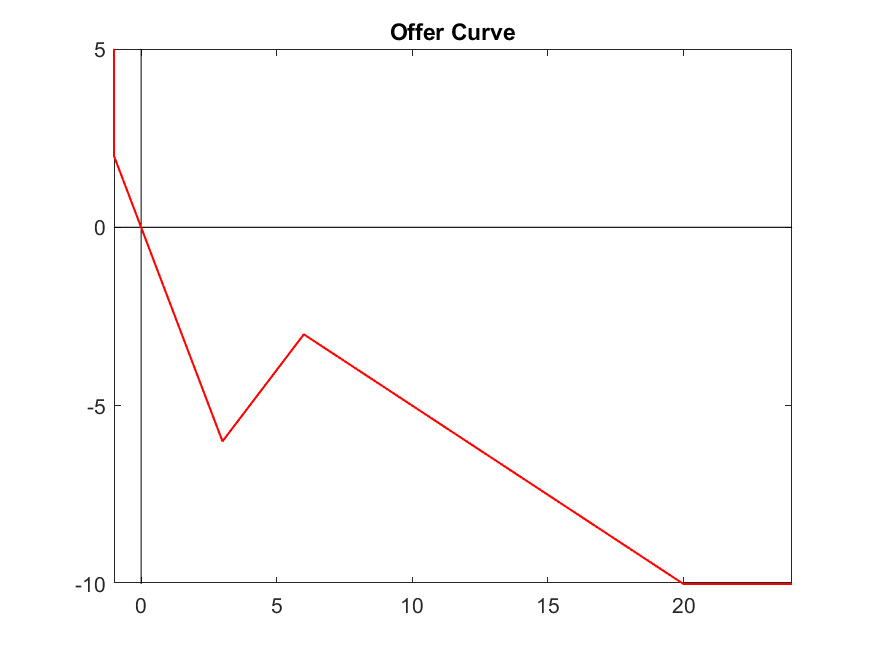
\includegraphics{off3}
%Our agent will trade to (weakly) increase their utility: $U(c_1,c_2)\geq U(w_1,w_2) = 12$. We will solve for a convenient expression for $c_1,c_2$:
%\begin{align*}
%2c_1 + c_2 &\geq 12 \\
%c_1 + 2c_2 &\geq 12 \\
%\Rightarrow  c_2&\geq 12 - 2c_1 \\
%\Rightarrow c_2&\geq \frac{12-c_1}{2}
%\end{align*}
%As in the previous subsection, we find that our agent will trade to any point which is on or above both curves. This is plotted below. Note: $c_1,c_2\geq 0.$
%
%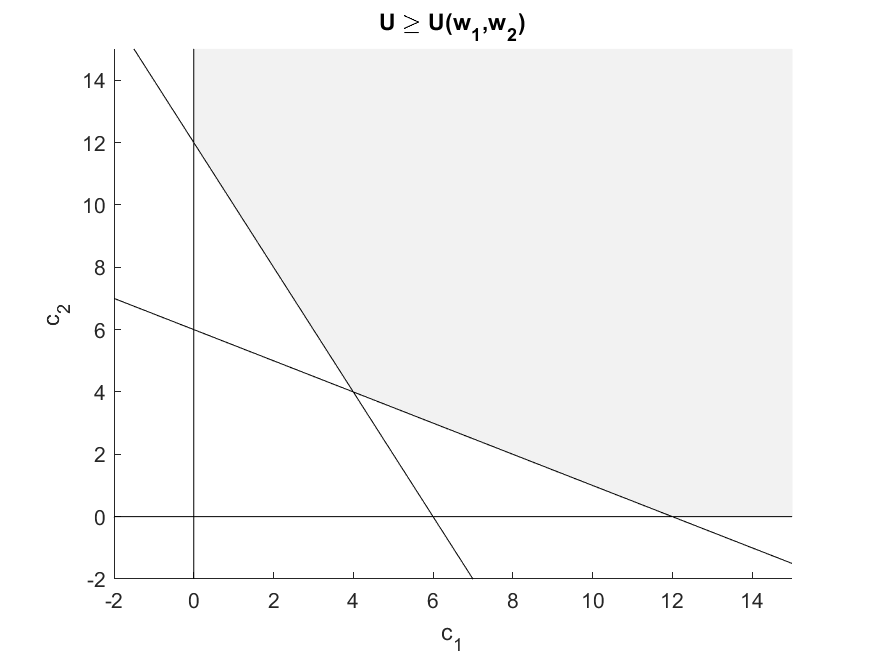
\includegraphics{p3}

\end{document}
